\chapter{Diseño en detalles}
\label{disenioEnDetalles}

\section{Diagrama de Clases de Remo}
\begin{figure}[!hbtp]
	\begin{center}
		\hspace*{-1.5cm}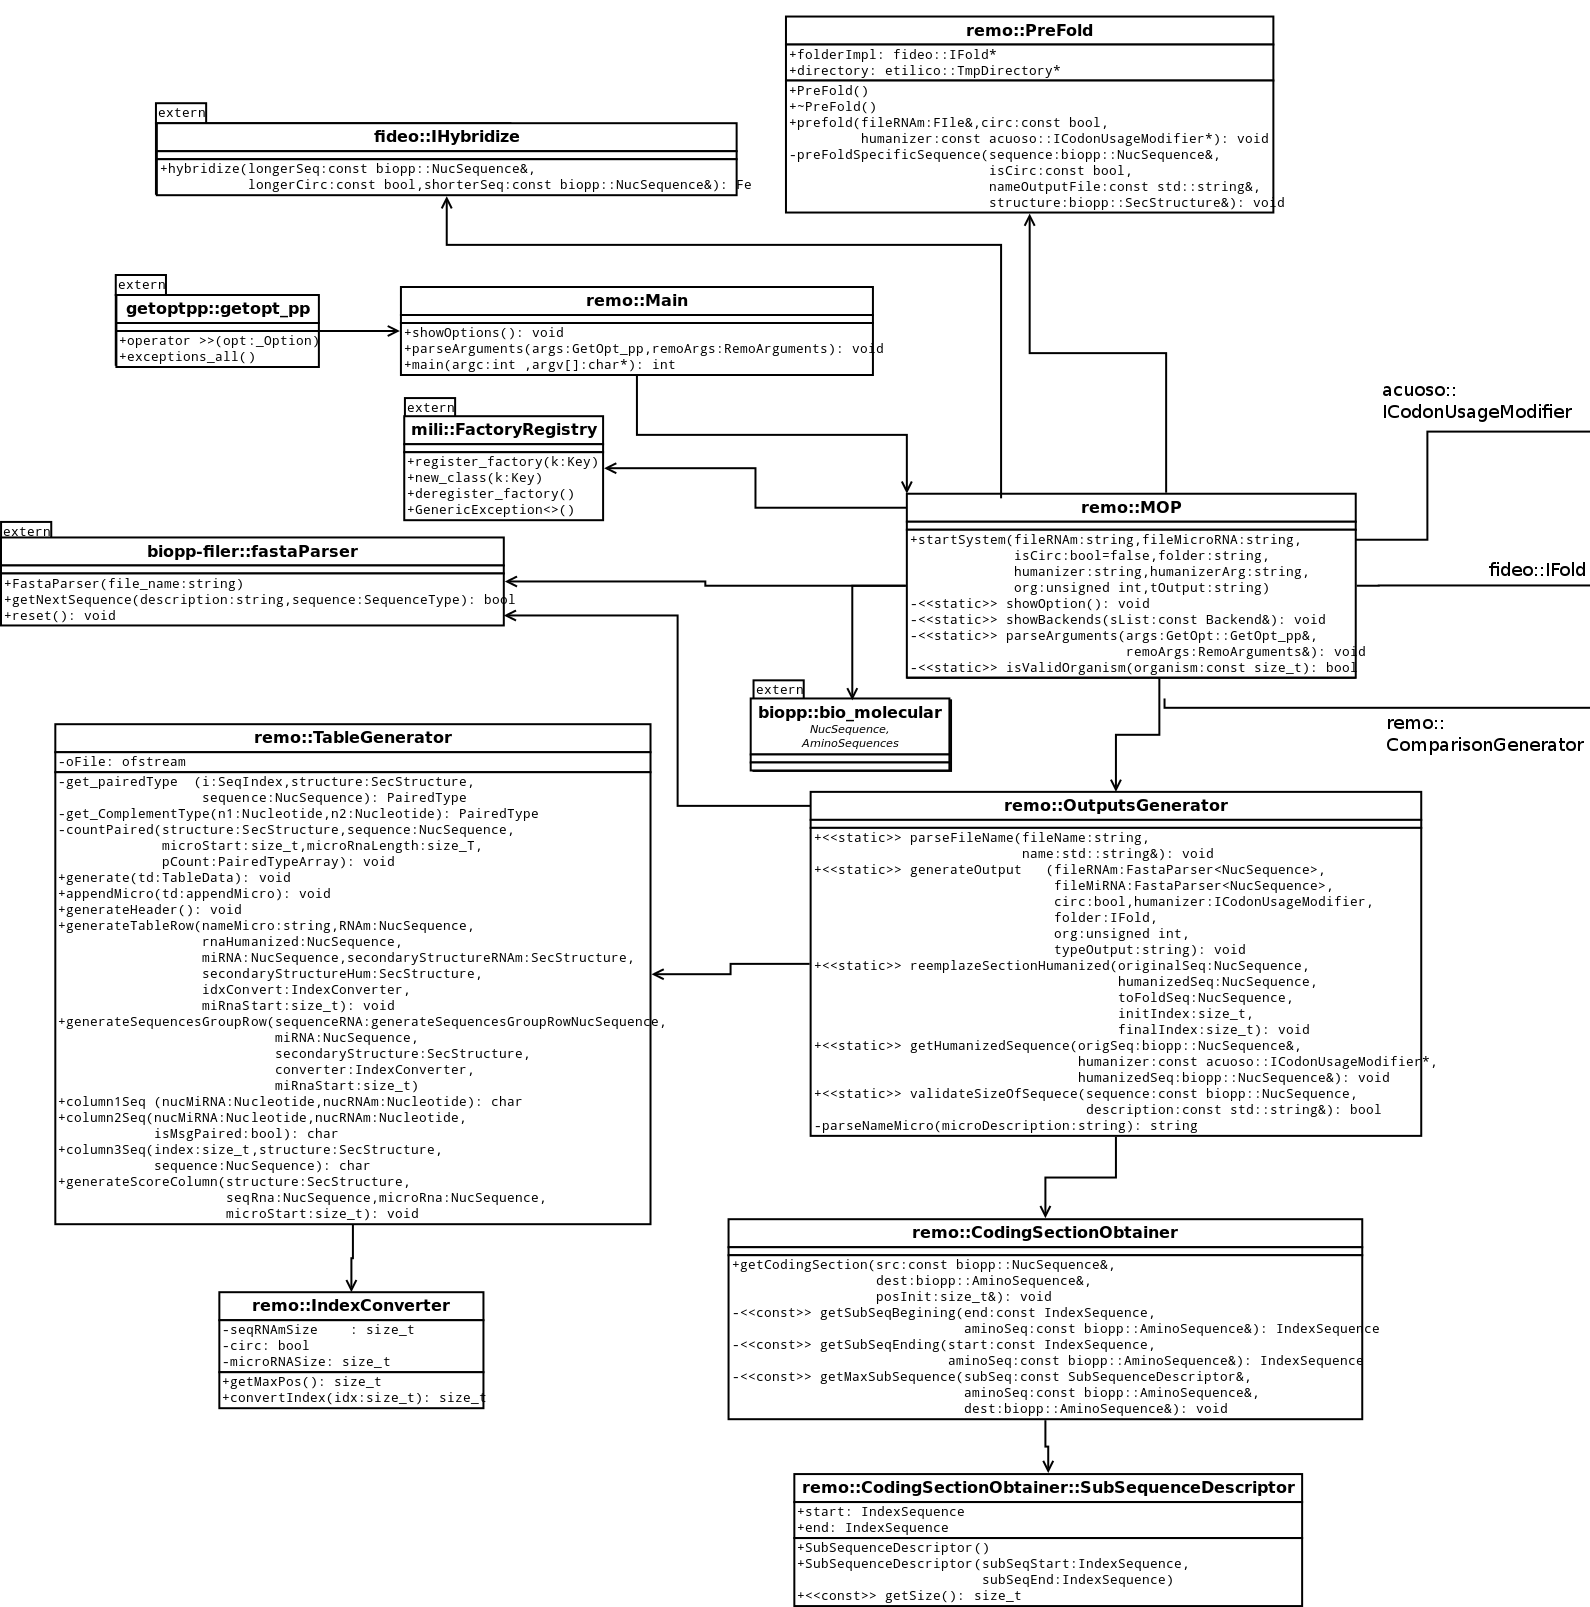
\includegraphics[width=20cm, height=17.5cm, angle=90]{image/remo1.png}
		\caption{UML - Diagrama de clases de \textbf{Remo}, parte 1 de 2 [2].}
		\label{remoDClase1}
	\end{center}
\end{figure}

\begin{figure}[!hbtp]
	\begin{center}
		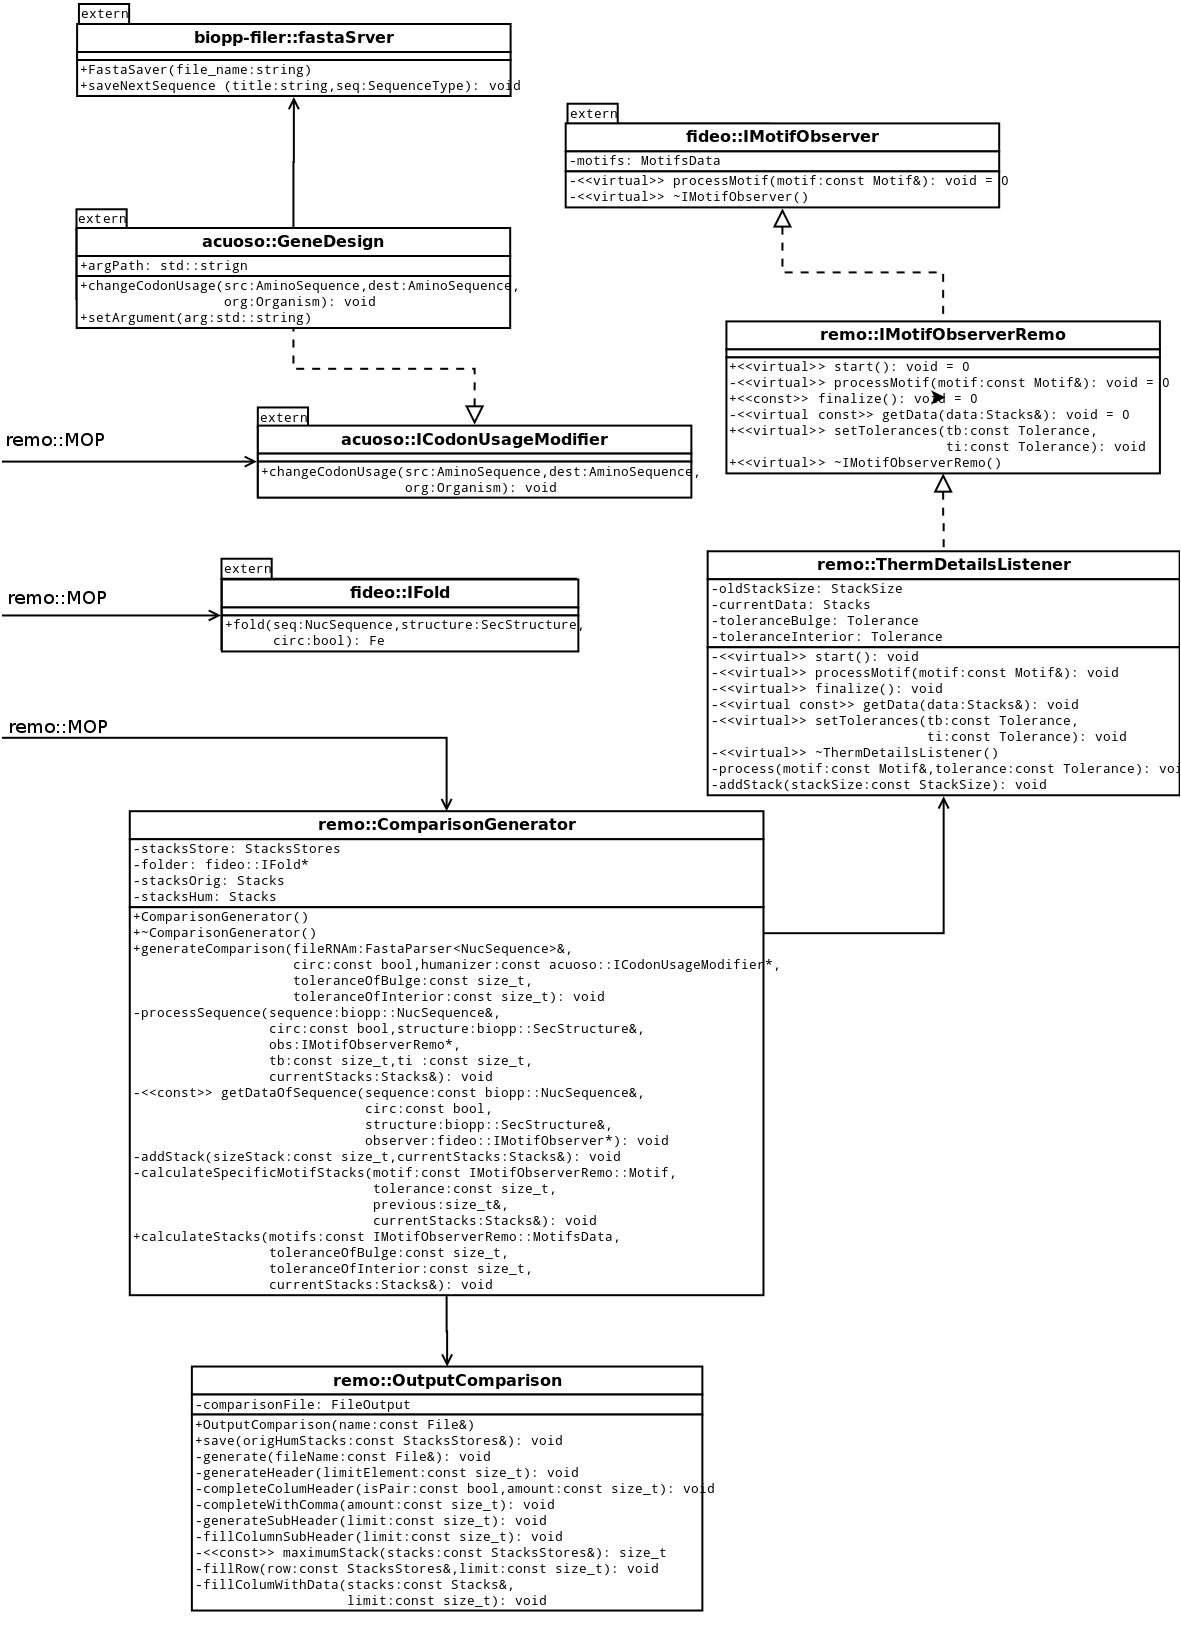
\includegraphics[width=16.5cm, height=18cm]{image/remo2.png}
		\caption{UML - Diagrama de clases de \textbf{Remo}, parte 2 de 2 [2].}
		\label{remoDClase2}
	\end{center}
\end{figure}

\section{Diagrama de Clases de Fideo}

\begin{figure}[!hbtp]
	\begin{center}
		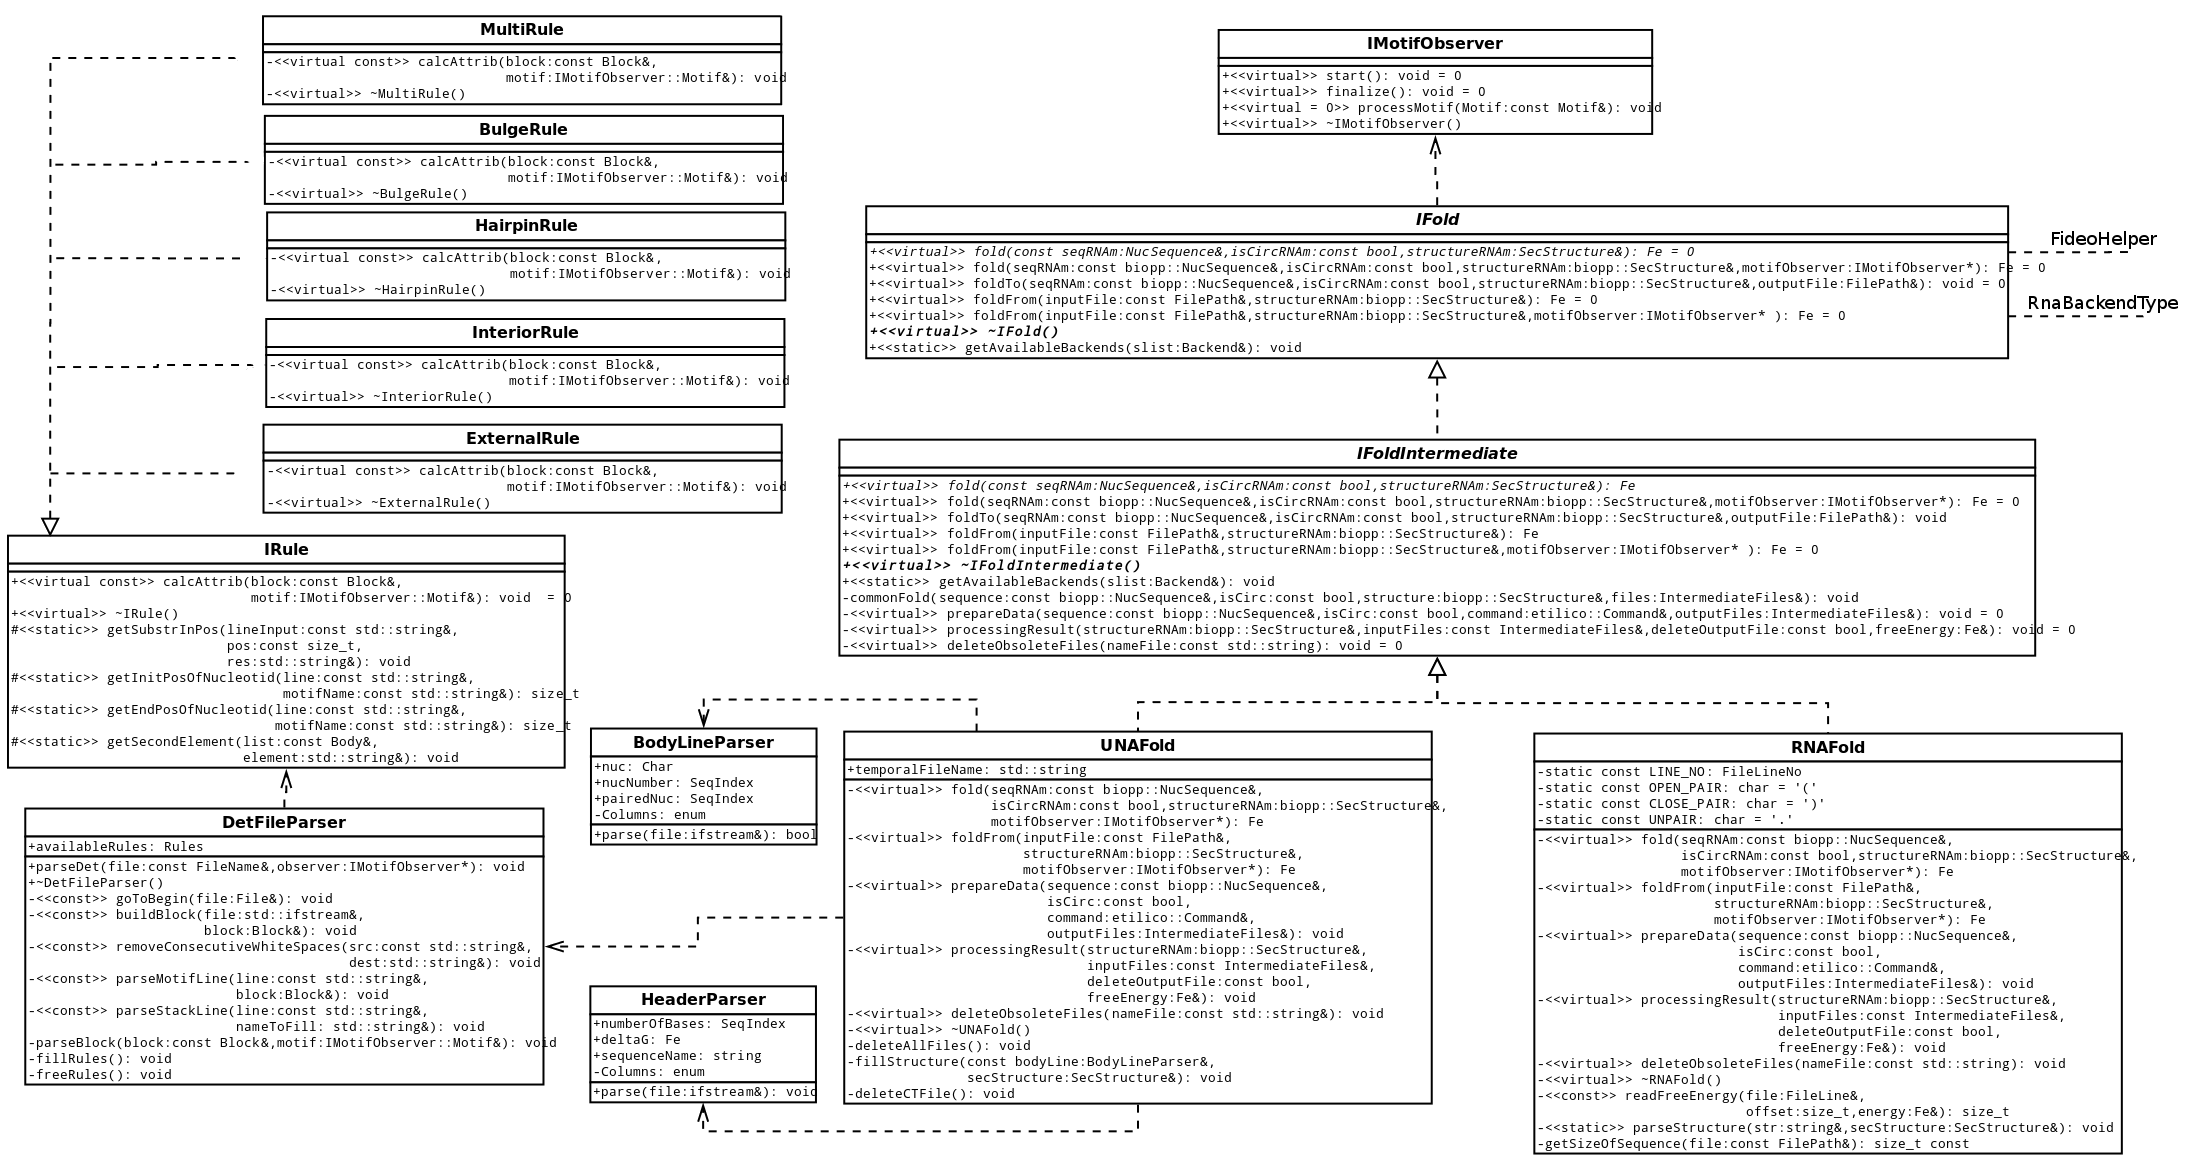
\includegraphics[width=20.5cm, height=13cm, angle=90]{image/fideoclass1.png}
		\caption{UML - Diagrama de clases de fideo, parte 1 de 2 [2].}
		\label{fideoDisenio1}
	\end{center}
\end{figure}

\begin{figure}[!hbtp]
	\begin{center}
		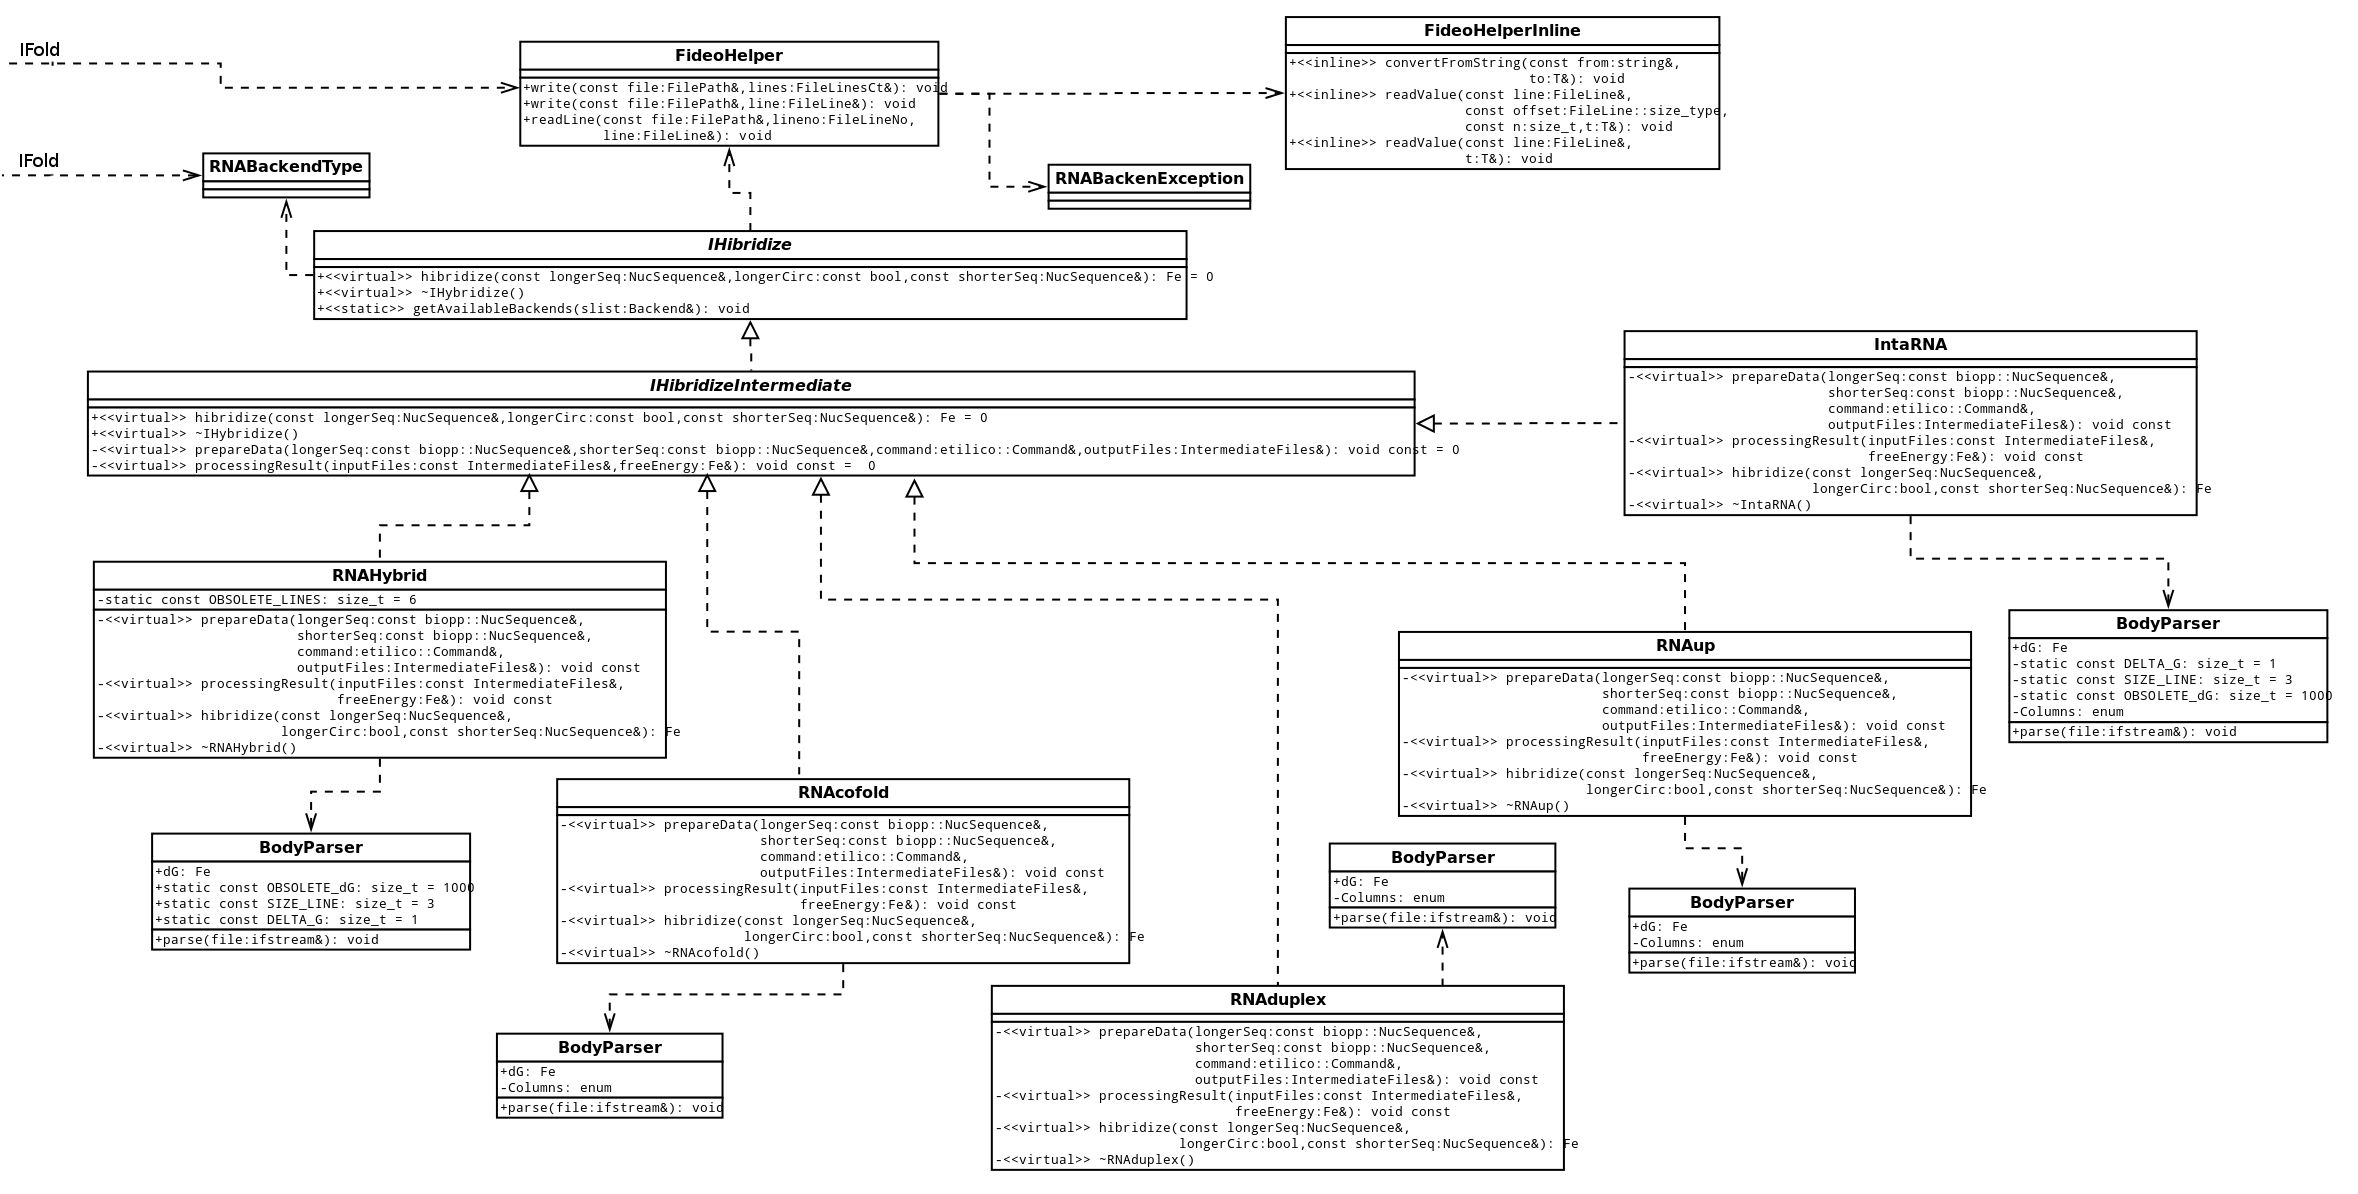
\includegraphics[width=20.5cm, height=12.5cm, angle=90]{image/fideoclass2.png}
		\caption{UML - Diagrama de clases de fideo, parte 2 de 2 [2].}
		\label{fideoDisenio2}
	\end{center}
\end{figure}